%!TEX program = lualatex
\documentclass[a4paper,12pt,openany,oneside]{memoir}

\usepackage{microtype}
\usepackage[hmargin = 1.91cm, vmargin = 2.54cm]{geometry}
\usepackage{float}

\usepackage[no-math]{fontspec}
\setmainfont{STIXTwoText}[
    Path            = ./fonts/STIX2/   ,
    UprightFont     = *-Regular.otf    ,
    BoldFont        = *-Bold.otf       ,
    ItalicFont      = *-Italic.otf     ,
    BoldItalicFont  = *-BoldItalic.otf
    ]

\usepackage{unicode-math}
\setmathfont{STIXTwoMath.otf}[Path = ./fonts/STIX2/]

\setmonofont{FiraCode}[
    Path        = ./fonts/FiraCode/ ,
    UprightFont = *-Regular.ttf    ,
    BoldFont    = *-Bold.ttf     ,
    ]

\usepackage[usenames,svgnames]{xcolor}
\usepackage{icomma}
\usepackage{tocloft}
\usepackage{hyperref}
\usepackage{enumitem} 
\makeatletter
\AddEnumerateCounter{\asbuk}{\russian@alph}{щ}
\makeatother
\usepackage{amsmath}
\usepackage{graphicx}
\usepackage{listings}
\usepackage[english,russian]{babel}


% Chapter header format
\renewcommand{\afterchapternum}{\hspace{1ex}}
\renewcommand{\chapnamefont}{\centering\bfseries\LARGE}
\renewcommand{\chapnumfont}{\centering\bfseries\LARGE}
\renewcommand{\chaptitlefont}{\centering\bfseries\LARGE}
\sethangfrom{\noindent #1}
\indentafterchapter

% Correct display of the new chapter and section formats with babel
\addto\captionsrussian{
    \renewcommand{\secheadstyle}{\centering\bfseries\Large\S\space}
    \renewcommand{\subsecheadstyle}{\centering\bfseries\large}
    \renewcommand{\contentsname}{\bfseries Содержание}
    \renewcommand{\chaptername}{\S}
    }
    
\pagestyle{plain}
\OnehalfSpacing

% Define new language style for C++
\lstdefinestyle{MyCPP}{
    language=C++ ,
    escapechar=\@ ,
    breaklines ,
    resetmargins=true ,
    keepspaces=true ,
    basicstyle=\ttfamily\small ,
    keywordstyle=\color{NavyBlue}\bfseries\ttfamily\small ,
    stringstyle=\color{Blue}\ttfamily\small ,
    commentstyle=\color{Green}\ttfamily\small ,
    morecomment=[l][\color{LimeGreen}]{\#} ,
    emph=[1]{cout,endl,std,string,ofstream,ifstream} ,
    emphstyle=[1]\color{ForestGreen}\bfseries\ttfamily\small ,
    literate=
        *{0}{{{\color{Magenta}0}}}1
        {1}{{{\color{Magenta}1}}}1
        {2}{{{\color{Magenta}2}}}1
        {3}{{{\color{Magenta}3}}}1
        {4}{{{\color{Magenta}4}}}1
        {5}{{{\color{Magenta}5}}}1
        {6}{{{\color{Magenta}6}}}1
        {7}{{{\color{Magenta}7}}}1
        {8}{{{\color{Magenta}8}}}1
        {9}{{{\color{Magenta}9}}}1
        {(}{{{\color{Red}(}}}1
        %fix right parenthesis ) not being colored
        {')}{{{\color{Red})}}}1
        %
        {[}{{{\color{Red}[}}}1
        {]}{{{\color{Red}]}}}1
        {=}{{{\color{Red}=}}}1
        {;}{{{\color{Red};}}}1
        {<}{{{\color{Red}<}}}1
        {.}{{{\color{Red}.}}}1
        {>}{{{\color{Red}>}}}1
        {+}{{{\color{Red}+}}}1
        {-}{{{\color{Red}-}}}1
        {*}{{{\color{Red}*}}}1
        {\&}{{{\color{Red}\&}}}1
        {\%}{{{\color{Red}\%}}}1
}

\begin{document}
% New section numbering format
\setsecnumformat{\csname the#1\endcsname \space}
% Quick command for using mono bold font
\newcommand{\monobf}[1]{{\ttfamily\textbf{#1}}}
% Set language style for C++
\lstset{style=MyCPP}

\tableofcontents*
\addcontentsline{toc}{chapter}{Предисловие}

\chapter{Установка редактора исходного кода Code::Blocks}
Для написания собственных программ на языке программирования C\texttt{++} необходимо установить любую из возможных сред разработки. Например, свободную кроссплатформенную среду разработки --- \textbf{Code::Blocks}.
\begin{itemize}
    \item Скачиваем дистрибутив с сайта {\color{Blue}\href{https://www.codeblocks.org/downloads/binaries/#imagesoswindows48pnglogo-microsoft-windows}{codeblocks.org}}.
    \item После установки на рабочем столе появляется иконка с одноименным названием, или же в меню \textbf{Пуск$\rightarrow$Все программы}.
    \item В открывшемся окне выбираем \textbf{Create a new project}
    \begin{figure}[H]
        \centering
        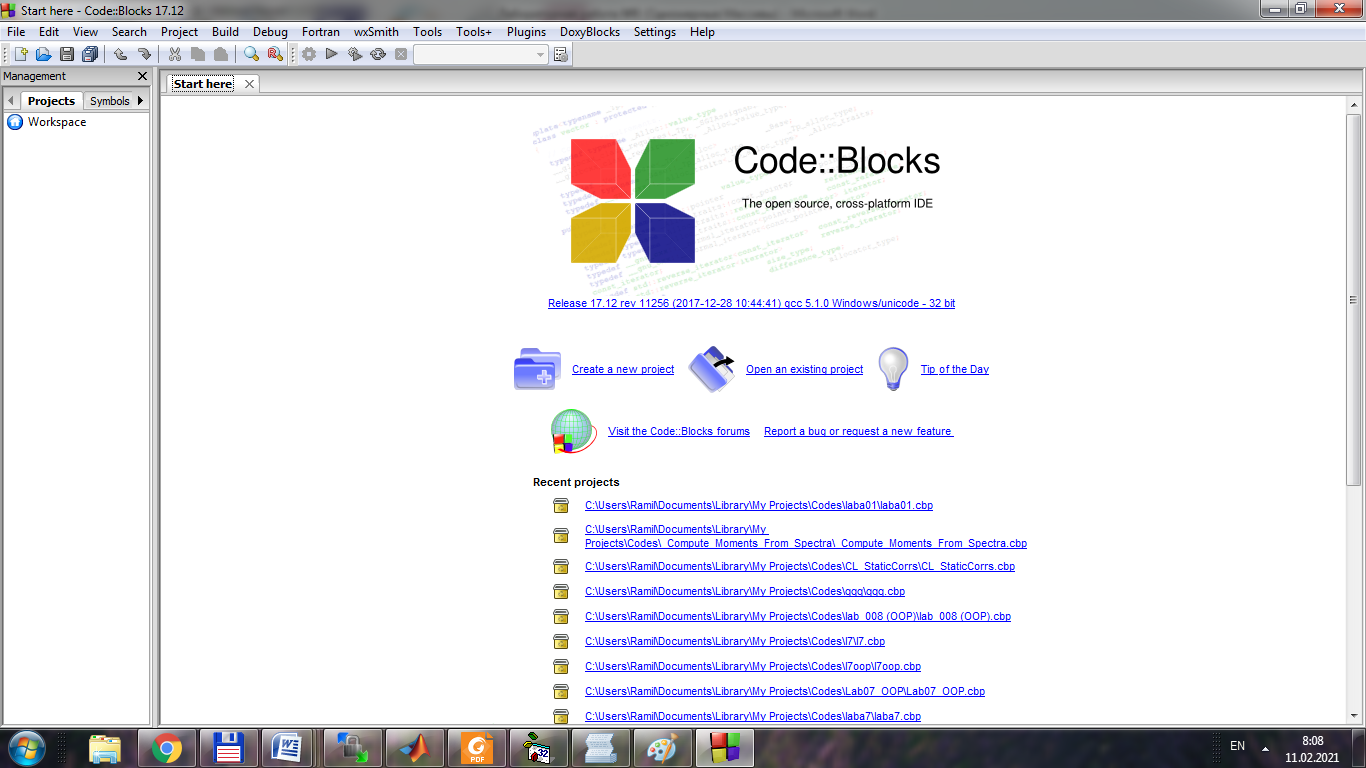
\includegraphics[width=.9\linewidth]{figures/CodeBlocks-1.png}
        \caption{Запуск программы Code::Blocks}
        \label{CodeBlocks-1}
    \end{figure}
    \item Выбираем иконку \textbf{Console Application}
    \begin{figure}[H]
        \centering
        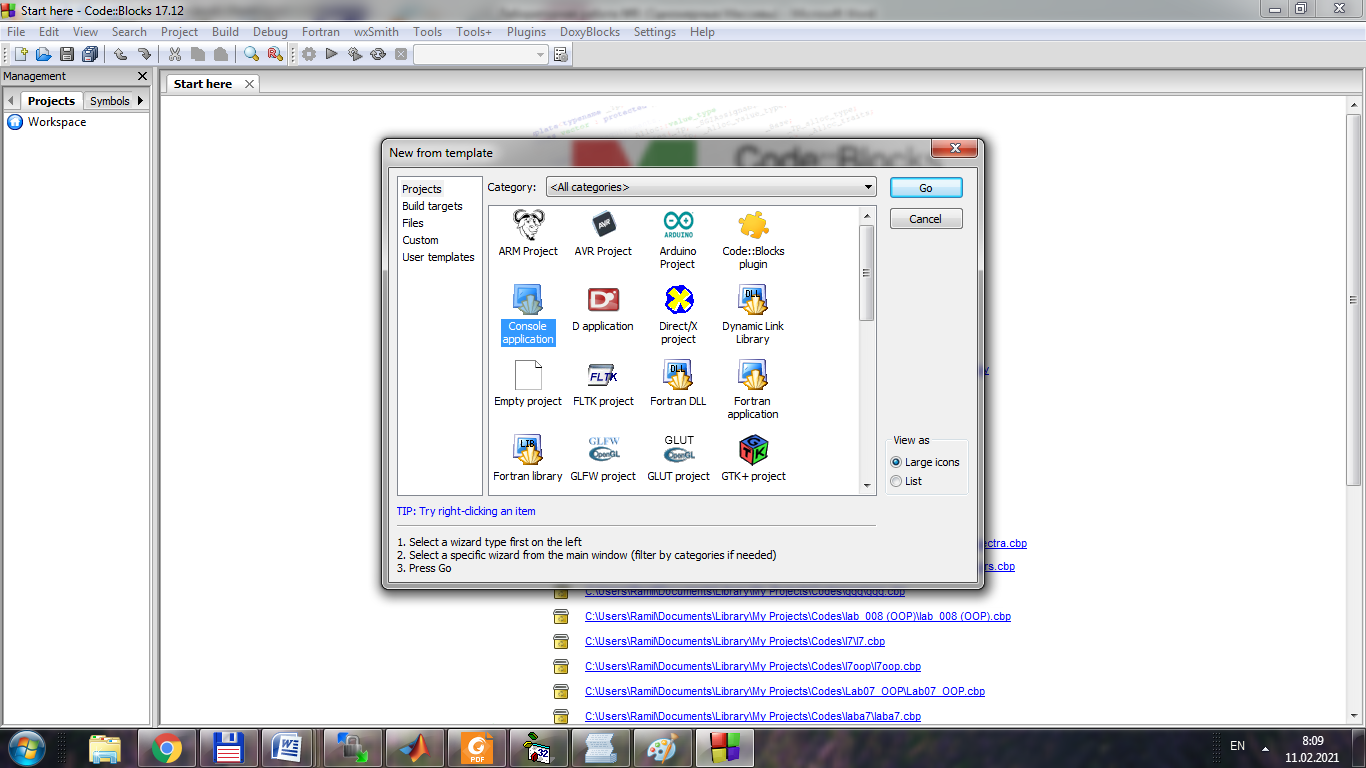
\includegraphics[width=.9\linewidth]{figures/CodeBlocks-2.png}
        \caption{Окно выбора иконки Console Application}
        \label{CodeBlocks-2}
    \end{figure}
    \item Выбираем \textbf{C\texttt{++}}
    \begin{figure}[H]
        \centering
        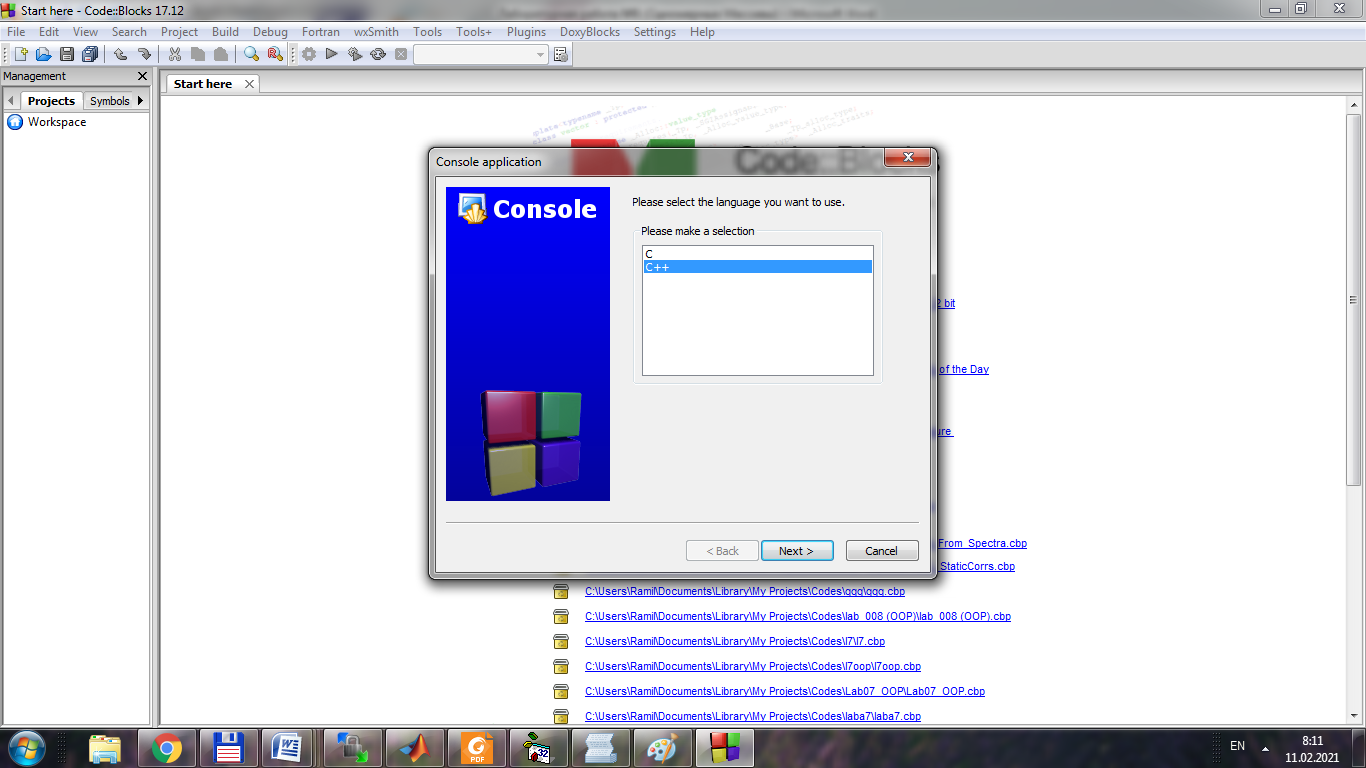
\includegraphics[width=.9\linewidth]{figures/CodeBlocks-3.png}
        \caption{Выбор языка C\texttt{++}}
        \label{CodeBlocks-3}
    \end{figure}
    \item Пишем имя проекта, например, \textbf{\_\_lab01}
    \begin{figure}[H]
        \centering
        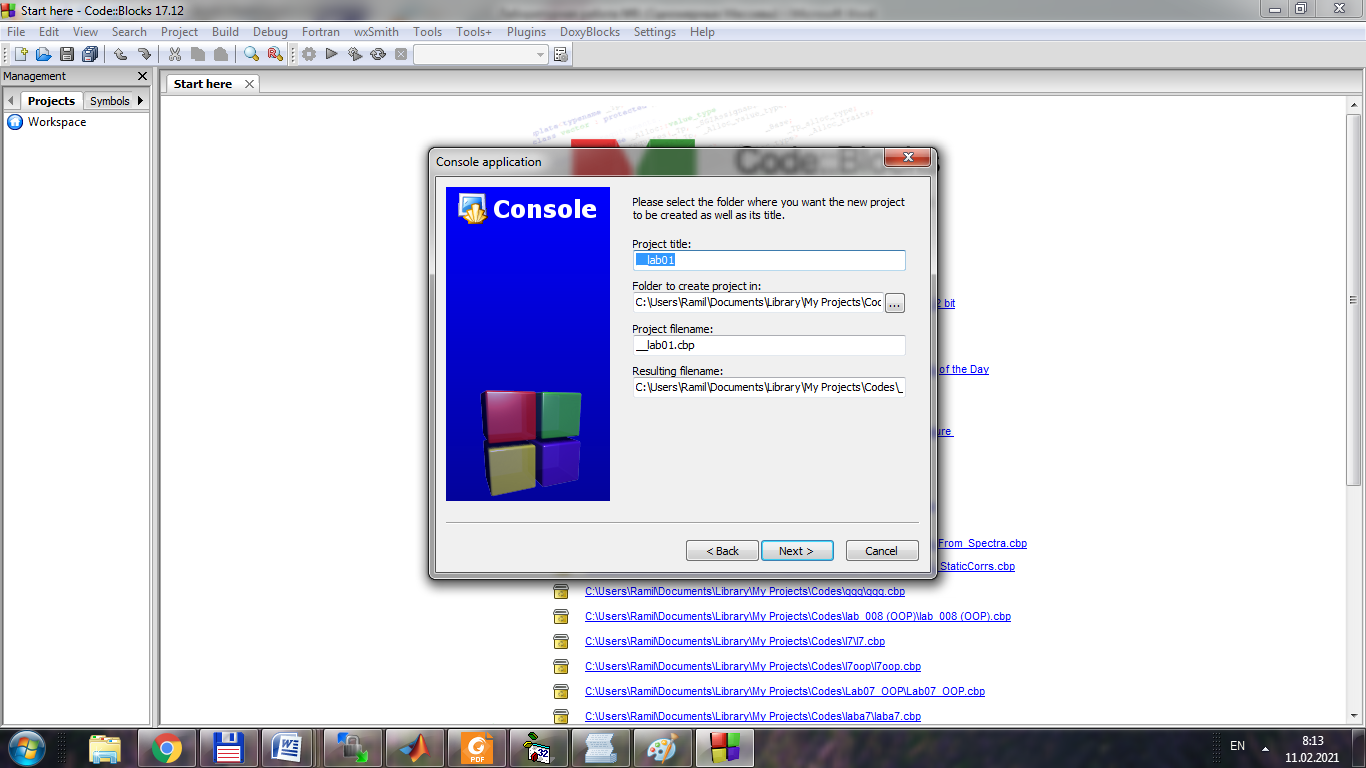
\includegraphics[width=.9\linewidth]{figures/CodeBlocks-4.png}
        \caption{Ввод имени проекта}
        \label{CodeBlocks-4}
    \end{figure}
    \item Далее, соглашаемся на все предложенные варианты, и кликаем на вкладку \textbf{Sources}$\rightarrow$ \textbf{main.cpp}. В результате, получаем следующее окно и шаблон программы \textbf{Hello, world!}
    \begin{figure}[H]
        \centering
        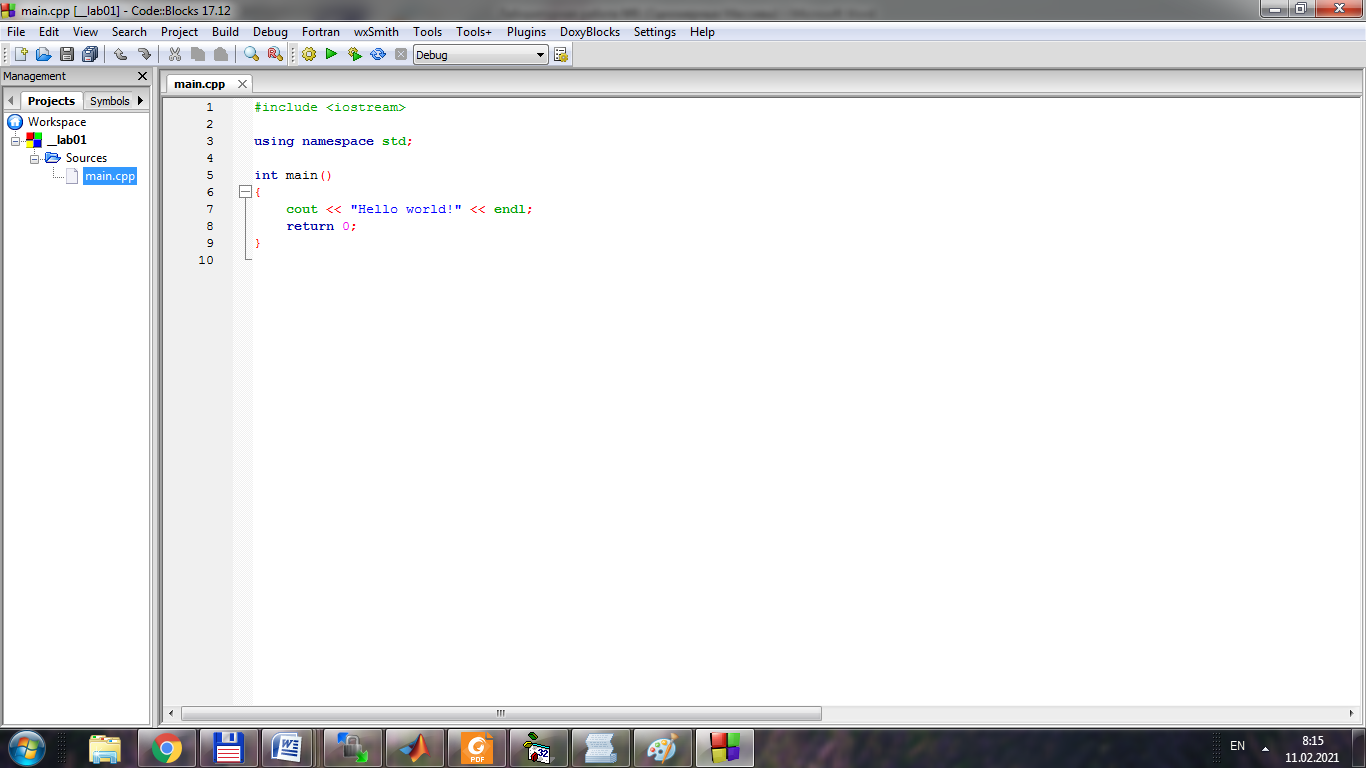
\includegraphics[width=.9\linewidth]{figures/CodeBlocks-5.png}
        \caption{Программа <<Hello, world!>> в окне редактора исходного кода}
        \label{CodeBlocks-5}
    \end{figure}
    \item Для компиляции и запуска программы нажимаем на клавишу \textbf{F9} (\textbf{Build and run}).
\end{itemize}
\chapter{Массивы}

\section{Одномерные массивы}
\begin{enumerate}[leftmargin=*]
    \item Дан массив вещественных чисел. Найдите сумму отрицательных элементов массива.
    \item Найдите произведение элементов массива с нечетными номерами.
    \item Дан массив целых чисел. Количество запросить с клавиатуры. Найти максимальный (минимальный) элемент массива и его номер, при условии, что все элементы различные.
    \item Найдите наименьший четный элемент массива. Если такого нет, то выведите первый элемент.
    \item Преобразовать массив так, чтобы сначала шли нулевые элементы, а затем все остальные.
    \item Ввести массив, в котором только два одинаковых элемента. Определить их местоположение.
    \item Ввести два массива действительных чисел. Определить максимальные элементы в каждом массиве и поменять их местами.
    \item Задан целочисленный массив. Определить процентное содержание элементов, превышающих среднеарифметическое всех элементов массива.
    \item Выполнить сортировку массива по возрастанию (убыванию).
    \item Дан массив из 10 элементов. Первые 4 упорядочить по возрастанию, последние 4 по убыванию.
\end{enumerate}
\section{Сортировка и упорядочение массивов}
\begin{enumerate}[leftmargin=*]
    \item Создайте матрицу случайных чисел размерности $n \times m$ в диапазоне $[1;10]$.
    \item Дана квадратная матрица. Вывести на экран элементы, стоящие на диагонали.
    \item Дана матрица. Вывести на экран все нечетные столбцы, у которых первый элемент меньше последнего.
    \item Дана матрица $N\times M$ случайных чисел. Отсортировать элементы главной диагонали матрицы по убыванию.
    \item Дана матрица $N\times M$ случайных чисел. Упорядочить первый столбец матрицы по возрастанию, а последний столбец --- по убыванию.
    \item Дан массив из 10 элементов. Отсортируйте отдельно элементы от 0-го по 2-й, с 3-го по 5-й и с 6-го по 9.
    \item Дан трехмерный массив $N\times M\times K$ случайных чисел $(N, M, K>5)$. Отсортируйте матрицу $N\times M$ при $K=2$ и выведите её на экран монитора.
    \item Дан массив 20 целых чисел на отрезке $[-2;5]$. Упорядочить массив, удалив нули со сдвигом влево, ненулевыми элементами.
    \item Дан массив 20 целых чисел на отрезке $[-5;5]$. Упорядочить массив, удалив повторяющиеся элементы.
    \item Дан массив. Найдите два соседних элемента, сумма которых минимальна.
    \item В данном массиве найдите количество чисел, соседи у которых отличаются более чем в 2 раза.
    \item Дана матрица. Вывести на экран все четные строки.
    \item Найдите сумму номеров минимального и максимального элементов массива.
    \item Введите одномерный целочисленный массив. Найдите наибольший нечетный элемент. Далее осуществите циклический сдвиг влево элементов, стоящих справа от найденного максимума.
    \item Дан массив размером nxn, элементы которого целые числа. Для каждого столбца подсчитать сумму отрицательных элементов и записать данные в текстовый файл.
    \item В двумерном массиве, элементы которого целые числа, удалить все столбцы, в которых первый элемент больше последнего. Результат записать в файл.
\end{enumerate}
\chapter{Файлы}
\section{Лабораторная работа 1}
\begin{enumerate}[leftmargin=*]
    \item Создайте матрицу \monobf{x[n][n]} случайных чисел. Сохраните все элементы матрицы в файл с названием \monobf{Matrix.txt}. Считайте содержимое файла \monobf{Matrix.txt} в новый массив \monobf{y[n][n]} и выведите его на экран дисплея.
    \item Напишите программу, которая считывала бы элементы главной диагонали матрицы из файла \monobf{Matrix.txt}.
    \item Напишите программу, которая удаляла бы $k$-столбец ($1<k<M$) в файле \monobf{Matrix.txt}.
    \item Напишите программу, которая считывала бы элементы матрицы из файла \monobf{Matrix.txt} и записывала бы их в массив, соответствующего размера. Отсортируйте все столбцы матрицы по убыванию. Полученный массив запишите в файл \monobf{Matrix\_Sort.txt}.
    \item Дан текстовый файл, содержащий целые числа. Удалить из него все четные числа. 
    \item В данном текстовом файле удалить все слова, которые содержат хотя бы одну цифру. 
    \item Напишите программу, которая считывала бы саму себя и выводила бы на экран дисплея исходный текст программы в обратном порядке.
    \item Имеется файл с текстом. Осуществить шифрование данного текста в новый файл. Осуществить расшифровку полученного текста.
\end{enumerate}
\chapter{Структуры}
\section{Лабораторная работа 1}
\begin{enumerate}[leftmargin=*]
    \item Описать структуру с именем \monobf{AEROFLOT}, содержащую следующие поля:
        \begin{itemize}
            \item название пункта назначения рейса;
            \item номер рейса;
            \item тип самолета.
        \end{itemize}
    \item Написать программу, выполняющую следующие действия:
        \begin{itemize}
            \item ввод с клавиатуры данных в массив, состоящий из семи элементов типа \monobf{AEROFLOT}; записи должны быть размещены в алфавитном порядке по названиям пунктов назначения (для этого выполните процедуру сортировки);
            \item вывод на экран пунктов назначения и номеров рейсов, обслуживаемых самолетом, тип которого введен с клавиатуры. Если таких рейсов нет, выдать на дисплей соответствующее сообщение.
        \end{itemize}
    \item Описать структуру с именем \monobf{STUDENT}, содержащую следующие поля:
        \begin{itemize}
            \item \monobf{NAME} – фамилия и инициалы;
            \item \monobf{GROUP} – номер группы;
            \item \monobf{SES} - успеваемость (массив из пяти элементов).
        \end{itemize}
    \item Написать программу, выполняющую следующие действия:
        \begin{itemize}
            \item ввод с клавиатуры данных в массив \monobf{STUD1}, состоящий из десяти структур типа \monobf{STUDENT}; записи должны быть упорядочены по возрастанию содержимого поля \monobf{GROUP};
            \item вывод на дисплей фамилий и номеров групп для всех студентов, включенных в массив, если средний балл студента больше 4,0. Если таких нет, вывести соответствующее сообщение.
        \end{itemize}
\end{enumerate}
\subsection{Лабораторная работа 2}
\begin{enumerate}[leftmargin=*]
    \item Информация об итогах сдачи сессии каждым студентом представлена в следующем порядке: Фамилия Имя Отчество, номер группы, экзаменационные оценки по четырем предметам. 
    Отсортируйте фамилии студентов по алфавиту. Определить процент студентов, сдавших экзамены на 4 и 5.
    \item Ведомость успеваемости студентов курса содержит следующую информацию: номер группы, фамилию, средний балл за последнюю сессию. Составить список студентов в порядке возрастания их номеров групп.
    \item Даны два отсчета времени в часах, минутах и секундах. Найти величину временного интервала в секундах. Код реализовать через составной тип данных.
    \item Дано пять различных дат в виде: число, месяц, год. Вывести их на экран в порядке возрастания.
    \item Создать массив структур для учета занятости аудитории: день недели, время учебной пары, аудитория, название предмета. Реализовать поиск периодов времени, когда выбранная аудитория свободна.
    \item Список книг содержит следующую информацию: фамилии авторов, название книги, год издания. Найти все книги, в названии которых имеется определенное слово, например, "физика".
    \item Список имеющихся в продаже автомобилей содержит следующие сведения: марка автомобиля, цвет, стоимость, мощность двигателя, расход бензина на 100 км. Вывести перечень автомобилей, удовлетворяющих определенным требованиям клиента, таким например, как стоимость в диапазоне 300-500 тыс.руб., расход бензина в пределах 8-10 л и т.п.
    \item Описать два комплексных числа и проделать над ними операции сложения, вычитания, умножения и деления.
\end{enumerate}

\chapter{Обработка строк}
\section{Лабораторная работа 1}
\begin{enumerate}[leftmargin=*]
    \item В заданном тексте заменить все символы <<+>> на << - >>. В данной задаче воспользуйтесь массивом символов (Заголовочный файл \monobf{\color{LimeGreen}cstring}).
    \begin{lstlisting}
        #include<iostream>
        #include<cstring>
        using namespace std;
        int main(')
        {   char str[50]="(5+3)*7+65+7896";
            cout << "Initial string is: " << str << endl;
            for (int i=0; i<strlen(str); i++')
                if (str[i] == '+'')
                    str[i] = '-';
            cout << "Final string is: " << str << endl;
            return 0;
        }
    \end{lstlisting}
    \item В данном тексте посчитать число символов <<+>> и <<->>.
    \item Напишите программу, которая вычисляет длину введенной с клавиатуры строки. Реализуйте код программы, используя строковый тип данных (Заголовочный файл \monobf{\color{LimeGreen}string}').
    \begin{lstlisting}
        #include <iostream>
        #include <string>
        using namespace std;
        int main(')
        {
            setlocale(LC_ALL,"Russian"');
            string s;
            cout <<" @\color{Blue}Введите строку@: \n"; cin >> s;
            cout <<" @\color{Blue}Строка@ " << s << " @\color{Blue}содержит@ "
                << s.length(') << " @\color{Blue}символ(а')@.\n";
            return 0;
        }
    \end{lstlisting}
    \item Задана строка символов. Определить, есть ли заданный символ «э» в этой строке символов. Выведите на экран номер первого вхождения данного символа в строке..
    \begin{lstlisting}
        #include <iostream>
        #include <string>
        using namespace std;
        int main(')
        {
            setlocale(LC_ALL,"Russian"');
            string str("@\color{Blue}Выведите на экран номер символа в строке@."');
            string symbol="@\color{Blue}э@";
            unsigned int pos str=str.find(symbol');
            if ((pos>=0') && pos(<str.length(')')')
                    cout << "@\color{Blue}Номер первого вхождения символа@ ("
                         << symbol << "') @\color{Blue}в строке@ \n\n("
                         << str << "')\n\n @\color{Blue}равен@: "<< pos << endl;
            else cout << "@\color{Blue}Такого символа в строке нет@!\n";
            return 0;
        }
    \end{lstlisting}
    \item Пусть задан некоторый текст. Вычислить, сколько раз повторяется наперед заданный символ <<\textbf{a}>>.
    \item Задана некоторая строка символов. Создать новую строку, которая образована из данной строки чтением от конца до начала.
    \item Задано слово. Проверить, читается ли это слово слева направо и наоборот. \textit{Простейшие \textbf{слова-палиндромы}}: мим, дед, наган, заказ, кабак, казак, мадам, шалаш.
    \item Вводится строка слов, разделенных пробелами. Найти самое длинное слово и вывести его на экран. 
    \item Пусть имеется текстовый файл, содержащий несколько строк символов. Подсчитать число символов <<->> в этих строках.
    \item Задана строка символов. Подсчитать число слов в этой строке. Считать, что слова разделяются одним из символов << >> (пробел), <<,>> (запятая), <<.>> (точка).
    \item Пусть имеется текстовый файл, содержащий несколько предложений. Подсчитать количество предложений и слов в этом файле.
    \item Пусть имеется текстовый файл, содержащий несколько слов. Отсортировать эти слова в алфавитном порядке и записать их в другой текстовый файл.
    \item Написать программу замены данных в строке. Пусть:\\ \textcolor{Red}{A = ''123456789''};\\
    \textcolor{Blue}{B = ''67''};\\
    \textcolor{Green}{C = ''-Шестьдесят семь-''};\\
    Необходимо найти символы \textbf{"67"} (из строки B) и заменить их на \textbf{"-Шестьдесят семь-"} (из строки C) в строке A, где A в итоге должна содержать \textbf{"12345-Шестьдесят семь-89"}.
\end{enumerate}
\subsection{Функции работы со строками}
\begin{table}[H]
    \centering
    \renewcommand{\arraystretch}{2}
    \begin{tabular}{|m{0.31\textwidth}|m{0.63\textwidth}|}
    \hline
    \multicolumn{1}{|c|}{Методы класса \textcolor{Green}{\monobf{String}}} & \multicolumn{1}{c|}{Описание метода}\\
    \hline
    \monobf{s.length()} & Возвращает длину строки \texttt{s} \\
    \hline
    \monobf{s.substr(pos,length)} & возвращает подстроку из строки \texttt{s}, начиная с номера
    \monobf{pos} длиной \monobf{length} символов; \\
    \hline
    \monobf{s.empty()} & возвращает значение \texttt{true}, если строка \texttt{s} пуста, \texttt{false} — в противном случае; \\
    \hline
    \monobf{s.insert(pos, s1)} & вставляет строку \monobf{s1} в строку \texttt{s}, начиная с позиции \texttt{pos}; \\
    \hline
    \monobf{s.remove(pos,length)} & удаляет из строки \texttt{s} подстроку \monobf{length} длинной \monobf{pos} символов; \\
    \hline
    \monobf{s.find(s1, pos)} & возвращает номер первого вхождения строки \monobf{s1} в строку \texttt{s}, поиск начинается с номера \monobf{pos}, параметр \monobf{pos} может отсутствовать, в этом случае поиск идет с начала строки; \\
    \hline
    \monobf{s.findfirst(s1, pos)} & возвращает номер первого вхождения любого символа из строки \monobf{s1} в строку \texttt{s}, поиск начинается с номера \monobf{pos}, который может отсутствовать.\\ 
    \hline
    \end{tabular}
    \caption{Функции работы со строками}
    \label{table_string_methods}
\end{table}
\chapter{Динамические типы данных}
\section{Лабораторная работа 1}
\begin{enumerate}[leftmargin=*]
    \item Напишите программу, реализующую объявление, заполнение и удаление динамического массива. Программа также должна выполнять вывод массива на экран и запись его в текстовый (бинарный) файл.
    \item Реализуйте предыдущую задачу с помощью подпрограмм (процедур и функций).
    \item Дана динамическая матрица случайных чисел размерности $N\times N$ ($N>9$). Вычислите произведение всех элементов матрицы, у которых индексы строк и столбцов четные. Результат выведите на экран.
    \item Описать структуру с именем \monobf{STUDENT}, содержащую следующие поля:
        \begin{itemize}
            \item \monobf{NAME} – фамилия и инициалы;
            \item \monobf{GROUP} – номер группы;
            \item \monobf{SES} - успеваемость (массив из пяти элементов).
        \end{itemize}
    Реализовать программу, используя указатели на структуру. Запишите данные для 10 студентов в файл.
    \item Создать структуру <<Товар>>. Каждый товар должен иметь не менее 8 полей, например, название; описание; страна и город, где произведен товар; предприятие-производитель; категория товара (продукты, хозтовары, промтовары и т.д.); цена; вес и т.д. Заполнить динамический массив десятью товарами. Реализовать поиск в массиве по названию, по вхождению слов в описание и по диапазону цены товара.
    \item Объявите указатель на массив типа \monobf{double} и предложите пользователю выбрать его размер. Далее напишите четыре функции: первая должна выделить память для массива, вторая – заполнить ячейки данными, третья – показать данные на экран, четвертая – освободить занимаемую память. Для обхода массива использовать указатели (запрещено обращаться к элементам массива по индексам).
\end{enumerate}
\begin{lstlisting}
    #include <iostream>
    #include <fstream>
    #include <cstdlib>

    using namespace std;
    int main(')
    {
        ofstream out("Array.txt"');
        const int n=10; double* x;
        x = new double[n];
        for (int i=0; i<n; i++')
        {
            *(x+i)=rand()%10;
            cout << "x["<< i << "]=" << *(x+i') << "\t";
            out << *(x+i) << "\n";
        }
        cout << "\n"; delete[] x; out.close(');

        ifstream in("Array.txt"');
        double * y;
        y = new double[n];
        for (int i=0; i<n; i++')
        {
            in >> *(y+i);
            cout << "y["<< i << "]="<< *(y+i') << "\t";
        }
        delete[] y; in.close('); return 0;
    }
\end{lstlisting}
\vspace{5cm}
\begin{lstlisting}
    #include <iostream>
    #include <fstream>
    #include <cstdlib>
    using namespace std;

    double* init(int n');
    void data(int n, double* x');
    void print(int n, double* x');
    void write_file(int n, double* x');
    void del(double* x');

    int main(')
    {
        int n; cout << "Input n: "; cin >> n;
        double* x=init(n');
        data(n,x');
        print(n,x');
        write_file(n,x');
        del(x');
        return 0;
    }
    double* init(int n') { return new double[n]; }
    void data(int n, double* x') { for (int i=0; i<n; i++') x[i]=rand(')%10; }
    void print(int n, double* x') { for (int i=0; i<n; i++') cout << x[i] << "\t"; }
    void write_file(int n, double* x')
    {
        ofstream out ("Array.txt"');
        for (int i=0; i<n; i++') out <<"x[" << i <<"]=" << x[i] << "\n";
        out.close(');
    }
    void del(double *x') { delete[] x; }
\end{lstlisting}
\vspace{5cm}
\begin{lstlisting}
    #include <iostream>
    using namespace std;
    int main(')
    {
        const int n=8, m=8;
        int **matrix;
        matrix=new int*[n];
        for (int i=0; i<n; i++')
            matrix[i]=new int[m];

        for (int i=0; i<n; i++')
        {
            for (int j=0; j<n; j++')
            {
                matrix[i][j]=(i+j'); cout << matrix[i][j] << "\t";
            }
            cout << endl;
        }
        delete[] matrix;
        return 0;
    }
\end{lstlisting}
\chapter{Рекурсия}
\begin{enumerate}[leftmargin=*]
    \item Напишите программу определения факториала "!" для неотрицательных целых чисел, используя рекурсивную функцию.
    \item Возведение числа $n$ в степень $р$ — это умножение числа $n$ на себя $р$ раз. Напишите рекурсивную функцию с именем \monobf{power()}, которая в качестве аргументов принимает значение типа \monobf{double} для $n$ и значение типа \monobf{int} для $р$ и возвращает значение типа \monobf{double}. Напишите функцию \monobf{main()}, которая запрашивает у пользователя ввод аргументов для функции \monobf{power()}, и отобразите на экране результаты ее работы.
    \item Написать функцию, вычисляющую биномиальный коэффициент $C_n^k$, без использования операторов цикла.
    \item Напишите рекурсивную функцию для вычисления суммы первых $n$ элементов целочисленного динамического массива.
    \item Написать функцию, вычисляющую $\textbf{НОД}(a,b)$ для неотрицательных целых $a$ и $b$ (без циклов).
    \item Написать функцию, печатающую цифры десятичного представления своего неотрицательного целого параметра, разделяя их пробелами: а) в обычном порядке; б) в обратном порядке (то и другое — без циклов).
    \item Написать функцию, проверяющую правильность скобочной структуры, без циклов:
    допускаются только символы «(», «)» и «.» (последний означает конец строки);
    допускаются три вида скобок («()», «[]» и «\{\}»). Конец строки — «.»
\end{enumerate}
\chapter{Функции и указатели}
\section{Лабораторная работа 1. Указатели}
\begin{enumerate}[leftmargin=*]
    \item С одномерным массивом, состоящим из $n$ вещественных элементов, выполнить следующее: Преобразовать массив таким образом, чтобы сначала располагались все положительные элементы, а потом – все отрицательные (элементы, равные 0, считать положительными).
    \item С одномерным массивом, состоящим из $n$ вещественных элементов, выполнить следующее: Преобразовать массив таким образом, чтобы сначала располагались все элементы, целая часть которых лежит в интервале $[a,b]$, а потом – все остальные.
    \item С одномерным массивом, состоящим из n вещественных элементов, выполнить следующее: Преобразовать массив таким образом, чтобы сначала располагались все отрицательные элементы, а потом – все положительные (элементы, равные 0, считать положительными).
    \item С одномерным массивом, состоящим из $n$ вещественных элементов, выполнить следующее: Преобразовать массив таким образом, чтобы сначала располагались все элементы, целая часть которых не превышает 1, а потом – все остальные.
    \item С одномерным массивом, состоящим из $n$ вещественных элементов, выполнить следующее: Преобразовать массив таким образом, чтобы сначала располагались все элементы, отличающиеся от максимального не более чем на 20\%, а потом – все остальные.
    \item С одномерным массивом, состоящим из $n$ вещественных элементов, выполнить следующее: Заменить все отрицательные элементы массива их модулями и изменить порядок следования элементов в массиве на обратный.
    \item С одномерным массивом, состоящим из $n$ вещественных элементов, выполнить следующее: Сжать массив, удалив из него одинаковые элементы.  Освободившиеся в конце массива элементы заполнить нулями.
    \item С одномерным массивом, состоящим из $n$ вещественных элементов, выполнить следующее: Сжать массив, удалив из него все элементы, модуль которых не превышает 1.  Освободившиеся в конце массива элементы заполнить нулями.
    \item С одномерным массивом, состоящим из $n$ вещественных элементов, выполнить следующее: Сжать массив, удалив из него все элементы, модуль которых находится в интервале $[a,b]$.  Освободившиеся в конце массива элементы заполнить нулями.
    \item С одномерным массивом, состоящим из $n$ вещественных элементов, выполнить следующее: Преобразовать массив таким образом, чтобы сначала располагались все элементы, равные нулю, а потом – все остальные.
    \item С одномерным массивом, состоящим из $n$ вещественных элементов, выполнить следующее: Преобразовать массив таким образом, чтобы в первой его половине располагались элементы,  стоявшие в нечетных позициях, а во второй половине – элементы, стоявшие в четных позициях.
    \item С одномерным массивом, состоящим из $n$ вещественных элементов, выполнить следующее: Преобразовать массив таким образом, чтобы сначала располагались все элементы, модуль которых не превышает 1, а потом – все остальные.
    \item С одномерным массивом, состоящим из $n$ вещественных элементов, выполнить следующее: Преобразовать массив таким образом, чтобы элементы, равные нулю, располагались после всех остальных.
    \item С одномерным массивом, состоящим из $n$ вещественных элементов, выполнить следующее: Преобразовать массив таким образом, чтобы в первой его половине располагались элементы,  стоявшие в четных позициях, а во второй половине – элементы, стоявшие в нечетных позициях.
    \item С одномерным массивом, состоящим из $n$ вещественных элементов, выполнить следующее: Сжать массив, удалив из него все элементы, величина которых находится в интервале $[a,b]$. Освободившиеся в конце массива элементы заполнить нулями.
\end{enumerate}
\section{Лабораторная работа 2. Подпрограммы-функции}
\begin{enumerate}[leftmargin=*]
    \item Напишите функцию, которая возвращает большее значение из введенных пользователем.
    \item Напишите программу, содержащую функцию, которая возводит число $a$ в степень $b$. Причем $a$ и $b$ вводятся с клавиатуры.
    \item Напишите функцию, вычисляющую процент от числа. Например: \textit{321\% от числа 3 равен 9.63}.
    \item Сделайте программу, функция которой сравнивает введенные числа и результат выдает в виде знаков ">", "<" или "=".
    \item Написать функцию, вычисляющую корни квадратного уравнения. В качестве аргументов она принимает коэффициенты $(a, b, c)$, а возвращает значение по обстоятельству ($x_1$ и $x_2$, либо «Корней нет», либо $а=0$ «Введены не корректные данные»).
    \item Напишите функцию, которая возвращает 1, если пользователь ввел гласную букву латинского алфавита, и 0 в противном случае.
    \item Написать функцию, специализированную на вывод строки из звездочек, количество которых определяется пользователем.
    \item Написать и протестировать функцию, которая из заданного массива формирует новый массив, состоящий только из элементов, дважды входящих в первый массив.
    \item Написать и протестировать функцию, возвращающую номер самого последнего элемента из массива, который совпадает с заданным с клавиатуры числом. Если такого элемента нет, функция должна возвращать "–1".
\end{enumerate}
\section{Лабораторная работа 3. Функции, указатели}
\begin{enumerate}[leftmargin=*]
    \item Создайте программу, реализующую работу с динамическим массивом. Разработайте 4 функции: первая - инициализация массива с выделением памяти под массив, вторая – заполнение массива данными, третья – вывод данных на экран, четвертая – освобождение занимаемой массивом памяти. 
    \item В целочисленном динамическом массиве \monobf{x[20]} определить сумму положительных элементов, делящихся на 5 без остатка и поставить ее на место максимального элемента массива \monobf{y[10]}. Реализуйте в виде отдельных функций: 1) создание массивов; 2) поиск элементов массива \monobf{x[20]}; 3) замена соответствующего элемента массива \monobf{y[10]}; 4) освобождение занимаемой массивами памяти.
    \item Программа. Описать функцию $f(x, n, p)$, определяющую, чередуются ли положительные и отрицательные элементы в целочисленном динамическом массиве \monobf{x[n]} из $n$ элементов и вычисляющую целочисленное значение $p$. Если элементы чередуются, то $p$ – это сумма положительных элементов, иначе $p$ – это произведение отрицательных элементов. С помощью этой функции провести анализ целочисленного массива \monobf{x[50]}.
    \item Создайте динамический массив случайных чисел. Перемешать его элементы случайным образом так, чтобы каждый элемент оказался на новом месте. Реализуйте программу в виде отдельных подпрограмм-функций.
    \item Дан динамический массив символов. Показать номера символов, совпадающих с последним символом строки. Реализуйте программу в виде отдельных подпрограмм-функций.
\end{enumerate}
\chapter{ООП}
\section{Лабораторная работа 1}
\begin{enumerate}[leftmargin=*]
    \item Создать класс \monobf{Employee}. Класс должен включать помимо имени и фамилии, поле типа \monobf{int} для хранения номера сотрудника и поле типа \monobf{float} для хранения величины его оклада. Методы класса должны позволять пользователю вводить и отображать данные класса. Написать функцию \monobf{main()}, которая запросит пользователя ввести данные для трех сотрудников и выведет полученную информацию на экран.
    \item Создать класс типа круг. Поля-данные: радиус, координаты центра. Функции-члены вычисляют площадь, длину окружности, устанавливают поля и возвращают значения. Функции-члены установки полей класса должны проверять корректность задаваемых параметров (не равны нулю и не отрицательные).
    \item Создать класс типа время с полями: час (0–23), минуты (0–59), секунды (0–59). Класс имеет конструктор. Функции-члены установки времени, получения часа, минуты и секунды, а также две функции-члены печати: печать по шаблону «16 часов 18 минут 3 секунды» и «4 p.m. 18 минут 3 секунды». Функции-члены установки полей класса должны проверять корректность задаваемых параметров.
    \item Создать класс типа дата с полями: день (1–31), месяц (1–12), год (целое число). Класс имеет конструктор. Функции-члены установки дня, месяца и года, функции-члены получения дня, месяца и года, а также две функции-члены печати: печать по шаблону «5 января 1997 года» и «05.01.1997». Функции-члены установки полей класса должны проверять корректность задаваемых параметров.
    \item Создать класс одномерный массив целых чисел (вектор) с полями --- количество фактических элементов, массив (динамический). Функции-члены: обращения к отдельному элементу массива, вывода массива на экран, поэлементного сложения и вычитания со скаляром, вывода элемента по заданному индексу.
    \item Создать класс множество \monobf{Set}. Функции-члены реализуют добавление и удаление элемента, пересечение и разность множеств.
\end{enumerate}

section{Лабораторная работа 2}
\begin{enumerate}[leftmargin=*]
    \item Создайте класс \monobf{Number}. Добавьте внутри класса функцию (метод) ввода переменной с клавиатуры и функцию вывода данной переменной на экран. Организуйте конструктор и деструктор с соответствующим выводом на экран сообщений \textbf{<<Сработал конструктор!>>} и <<Сработал деструктор!>>.
    \item Измените предыдущую программу таким образом, чтобы класс \monobf{Number} состоял из двух полей: целочисленной и символьной переменных. Организуйте работу деструктора и 4 конструкторов: конструктор без параметров, конструктор с целочисленным параметром, конструктор с символьным параметром, конструктор с обоими параметрами. 
    \item Создайте класс \monobf{Children}, который содержит такие поля (члены класса): закрытые (\monobf{private}) – имя, отчество и фамилию ребенка, а также его возраст; публичные (\monobf{public}) – методы ввода данных и отображения их на экран. Объявить два объекта класса, внести данные и показать их. Организуйте конструктор и деструктор с соответствующим выводом на экран сообщений \textbf{<<Сработал конструктор!>>} и \textbf{<<Сработал деструктор!>>}.
    \item Создать класс типа параллелепипед. Поля – высота, длина и ширина. Функции-члены вычисляют площадь и объем, сумму длин всех ребер параллелепипеда и длину главной диагонали, устанавливают поля и возвращают значения. Функции-члены установки полей класса должны проверять корректность задаваемых параметров (не равны нулю и не отрицательные). Организуйте два вида конструктора: без параметров и с параметрами по умолчанию, а также деструктор с сообщением об уничтожении объекта.
    \item Создайте класс <<Книга>>, содержащий следующие поля: название, количество страниц, год издания, цена. Методы: вычисления средней стоимости страницы; сколько лет книги; определение количества дней, прошедших после года издания книги. Создайте для данного класса конструктор и деструктор.
    \item Создайте класс одномерный динамический массив \monobf{Array}, который содержит такие поля (члены класса): публичные – методы ввода данных и отображения их на экран, а также определение максимального элемента массива. Создайте для данного класса конструктор и деструктор.
    \item Создайте класс \monobf{Matrix}, который содержит такие поля (члены класса): публичные – методы ввода данных и отображения их на экран, а также определение максимального элемента матрицы. Создайте для данного класса конструктор и деструктор.
\end{enumerate}
\chapter{Общие задачи}
\begin{enumerate}[leftmargin=*]
    \item Вычисление числа $\pi$. Для вычисления числа π используем ряд
    \begin{equation*}
        \frac{\pi}{4}=1-\frac{1}{3}+\frac{1}{5}-\frac{1}{7}+\frac{1}{9}-\dots .
    \end{equation*}
    Провести вычисления, обеспечив заранее заданную точность $\varepsilon>0$. При этом вычисления заканчиваются при $a < \varepsilon$.
    \item Напишите программу, которая находит факториал от введенного числа. Реализуйте алгоритм в виде рекурсивной функции.
    \item Определить число $e$ --- основание натуральных логарифмов с помощью ряда:
    \begin{equation*}
        e=1+\frac{1}{1!}+\frac{1}{2!}+\frac{1}{3!}+\frac{1}{4!}+\dots+\frac{1}{n!} .
    \end{equation*}
    Вычислить $е$ для всех значений $n$ от 1 до 20. Для каждого случая вывести на экран $n$ и соответствующее значение $е$.
    \item Дан текстовый файл $f$, компоненты которого являются целыми числами. Записать в файл $g$ все четные числа файла $f$, а в файл $h$ – все нечетные. Порядок следования чисел сохраняется.
    \item Ввести натуральное $N$ и проверить, является ли оно совершенным? Примечание: совершенное число равно сумме всех своих делителей, исключая само число. Например, 6 = 1 + 2 + 3.
    \item Составить программу для нахождения всех автоморфных чисел в отрезке $[m, n]$. Автоморфным называется целое число, которое равно последним числам своего квадрата. 
    \textit{Например:} 52 = 25, 62 = 36, 252 = 625.
    \item Известно, что сумма $N$ первых нечетных чисел равна квадрату числа $N$. Например, $1+3+5=3^2$, $1+3+5+7=4^2$ и т.д. Ввести натуральное К и распечатать таблицу всех натуральных чисел от $1$ до $К$ и их квадратов с использованием указанного соотношения.
    \item Дано натуральное число $n$ $(n≤100)$, определяющее возраст человека (в годах). Дать для этого числа наименования «год», «года», или «лет». Например, 1 год, 23 года, 45 лет и т.д.
    \item Написать программу вычисления методом Монте-Карло площади фигуры, ограниченной половиной синусоиды.
    \item Задача на перебор. Получить все перестановки элементов $1, … , 6$.
    \item Написать программу для вычисления методом Монте-Карло площади $S$ тела, ограниченного кривыми $xy=a$ и $x+y=\frac{5}{2}a$. Сравнить результат с точным значением.
    \item Игра «Угадай число». Один из играющих задумывает число от 1 до 1000, другой пытается угадать его за десять вопросов вида: верно ли, что задуманное число больше такого-то числа. Написать программу, играющую за отгадчика.
    \item Пусть даны четыре целых числа \textit{(hour, min, sec, time)}. Первые три из них \textit{(hour, min, sec)} – это время запуска ракеты в часах, минутах и секундах. Четвертое \textit{(time)} –-- определяет время полета в секундах. Вычислить время возвращения ракеты на землю.
    \item Один из простейших способов шифровки текста состоит в табличной замене каждого символа другим символом --- его шифром. Выбрать некоторую таблицу, разработать способ ее представления, затем
    \begin{enumerate}[label=\asbuk*)]
        \item зашифровать данный текст;
        \item расшифровать данный текст.
    \end{enumerate}
    \item Численно решить уравнение радиоактивного распада:
    \begin{equation*}
        \dfrac{dN}{dt} = -\lambda N .
    \end{equation*}
    Разработать алгоритм решения  задачи и написать программу на языке программирования C\texttt{++}. Сравнить численное решение с аналитическим. Определить условия сходимости.
    \item Создать типизированный файл записей со сведениями о телефонах абонентов; каждая запись имеет поля: фамилия абонента, год установки телефона, номер телефона. По заданной фамилии абонента выдать номера его телефонов. Определить количество установленных телефонов с $N$-го года. Отсортировать список по алфавиту и вывести все записи на экран.
    \item Напишите функцию, которая преобразовывает значение, заданное в радианах, в значение, выраженное в градусах, угловых минутах и угловых секундах. Воспользуйтесь указателем на структурный тип данных.
    \item Напишите программу, которая считывает числовые значения из файла, вычисляет значение полусуммы наибольшего и наименьшего элементов, а затем подсчитывает количество значений, не превышающих по величине полусумму, и больших чем полусумма.
    \item Напишите программу, которая меняет местами столбцы матрицы, содержащие наибольший и наименьший элементы.
    \item Треугольник задан координатами трех своих вершин. Определить, где находится точка $О$ с указанными координатами - внутри или вне треугольника.
    \item Составьте алгоритм и напишите программу для вычисления приближенного значения натурального логарифма от произвольного значения аргумента $|x|<1$, вводимого с клавиатуры. Ряд Тейлора для этой функции имеет вид:
    \begin{equation*}
        ln(1+x)=x-\frac{x^2}{2!}+\frac{x^3}{3}-{x^4}{4}+\dots .
    \end{equation*}
    \item Напишите программу, которая "сжимает" текстовый файл, считывая его элементы и заменяя все повторяющиеся символы, например, \textbf{ccccc}.... текстом \textbf{c(n)}, где \textbf{n}-число повторений символа \textbf{c}. В программе используйте процедуры-функции.
\end{enumerate}

\end{document}